\section{Object Class Recognition}

Two main tasks: Classification and Detection

Classification: is there a car in this image ? A binary answer is enough\\
Detection: where is the car ? Need localization

\subsection{Bag of words approaches: Visual words}
\subsubsection{Local features}
Local (textured) patches (‘regions’) • Detection co-variant with translation, scale, and sometimes affine transformations
• Cover the same portion of the object in any view



Each patch / region has a descriptor, which is a point in some high-dimensional feature space (e.g., SIFT)

Close points in feature space have similar descriptors, which indicates similar image content.

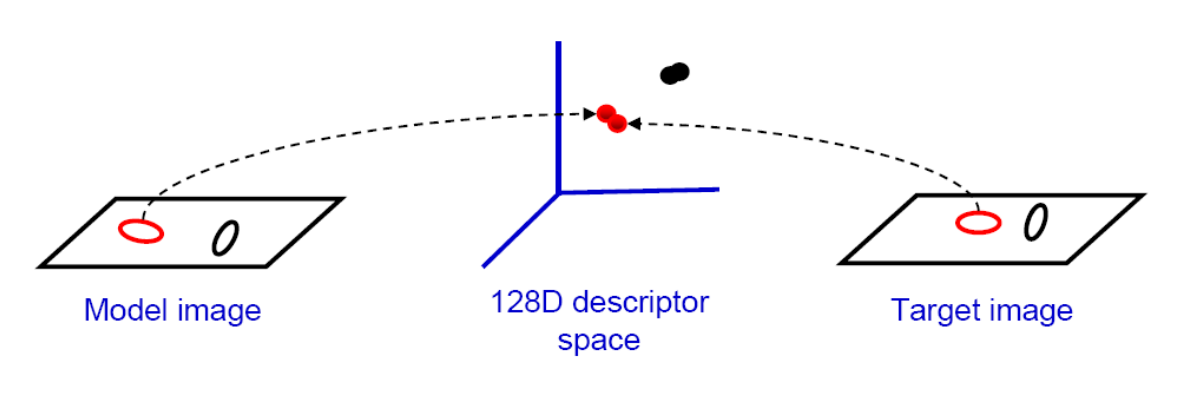
\includegraphics[width=\columnwidth]{pictures/localfeature}

\subsubsection{Visual Words}
1) Extract some local features from a number of images

2) Map high-dimensional descriptors to words by quantizing the feature space (Quantize via clustering, let cluster centers be the prototype “words”)

3) Map high-dimensional descriptors to words by quantizing the feature space. Determine which word to assign to each new image region by finding the closest cluster center

Building Visual Vocabularies
Issues: • Sampling strategy: where to extract features? ->
For object classes dense sampling works best
• Clustering / quantization algorithm ->
Many options, often k-means works well enough
• What corpus provides features (universal vocabulary?) ->
Typically as close as possible to your application • Vocabulary size, number of words\\

\subsection{Bag of Words}
Summarize entire image based on its distribution (histogram) of word occurrences.
(Analogous to bag of words representation commonly used for documents.) Quantize feature space to make discrete set of visual words

Bag of words enable to describe the unordered feature set with a single vector of fixed dimensionality

Works pretty well for whole-image classification

Classifier Choises

\begin{itemize}
	\item Nearest Neighbor
	\item Neural Networks
	\item Support Vector Machines
	\item Boosting
\end{itemize}

Nearest Neighbor - Assign label of nearest training data point to each test data point. Works very fast when training data is huge.
Support Vector Machines - Maximize the margin between the positive and negative training examples

The bag of words removes spatial layout. This is both a strength and a weakness

\subsubsection{Discussion: Bag-of-Words}
Pros:
\begin{itemize}
	\item Flexible to geometry / deformations / viewpoint
	\item Compact summary of image content
	\item Provides vector representation for sets (bags to be precise)
	\item Empirically good recognition results in practice
\end{itemize}
Cons:
\begin{itemize}
	\item Basic model ignores geometry – can verify afterwards, or embed within feature descriptors
	\item Background and foreground mixed when bag covers whole image - Interest points or sampling: no guarantee to capture object-level parts
	\item Optimal vocabulary formation remains unclear

\end{itemize}

\subsection{Classification: convolutional neural networks}
Neural network with specialized connectivity structure.

Typical building blocks of CNNs for classification in vision

\begin{itemize}
	\item Feed forward
	\item Most layers (often)
	\begin{itemize}
		\item Convolve input (filters)
		\item Non-linearity (rectified linear)
		\item Pooling (local max)
	\end{itemize}
	\item Last few layers (often)
	\begin{itemize}
		\item fully connected (linear combinations)
		\item Non-linearity (rectified linear)
	\end{itemize} 
	\item output: softmax distribution over classes
\end{itemize}
supervise, train convolutional filters by back-propagatin classification error


\subsection{Detection: Sliding-window approaches}
If object may be in a cluttered scene, slide a window around looking for it. - A brute force approach with many local decisions

\subsubsection{Gradient based Representations}
Summarize local distribution of gradients with histogram

\subsection{Boosting}
Intuition
Consider a 2D feature
space with positive and negative examples.
Each weak classifier splits the training examples with at least 50% accuracy.
Examples misclassified by a previous weak learner are given more emphasis at future rounds. Final classifier is combination of the weak classifiers

\subsection{Discussion: Sliding-Windows }
Pros
\begin{itemize}
	\item Simple detection protocol to implement
	\item Good feature choices critical
	\item Past successes for certain classes
	\item Good detectors available (Viola\&Jones, HOG, etc.)
\end{itemize}
Cons/Limitations
\begin{itemize}
	\item High computational complexity 
	\begin{itemize}
		\item – For example: 250,000 locations x 30 orientations x 4 scales = 30,000,000 evaluations!
		\item This puts tight constraints on the classifiers we can use.
		\item If training binary detectors independently, this means cost increases linearly with number of classes.
	\end{itemize}
	\item With so many windows, false positive rate better be low
	\item Typically need fully supervised training data (= bounding-boxes)
	\item Some object do not fit a box well (diagonal bottle) Sensitive to partial occlusion (unless in training data)
\end{itemize}

\subsection{Detection: proposal-based approaches}
\subsubsection{Object proposals}
Every object has at least one of these properties
• Well-defined, closed boundary in space • Different appearance than its surroundings • Might be unique within the image (salient)

Objectness(w) = probability that w covers an object

Objectness cues
\begin{itemize}
	\item Density of salient pixels
	\item color contrast
	\item superpixel straddling
\end{itemize}
\subsubsection{R-CNN}
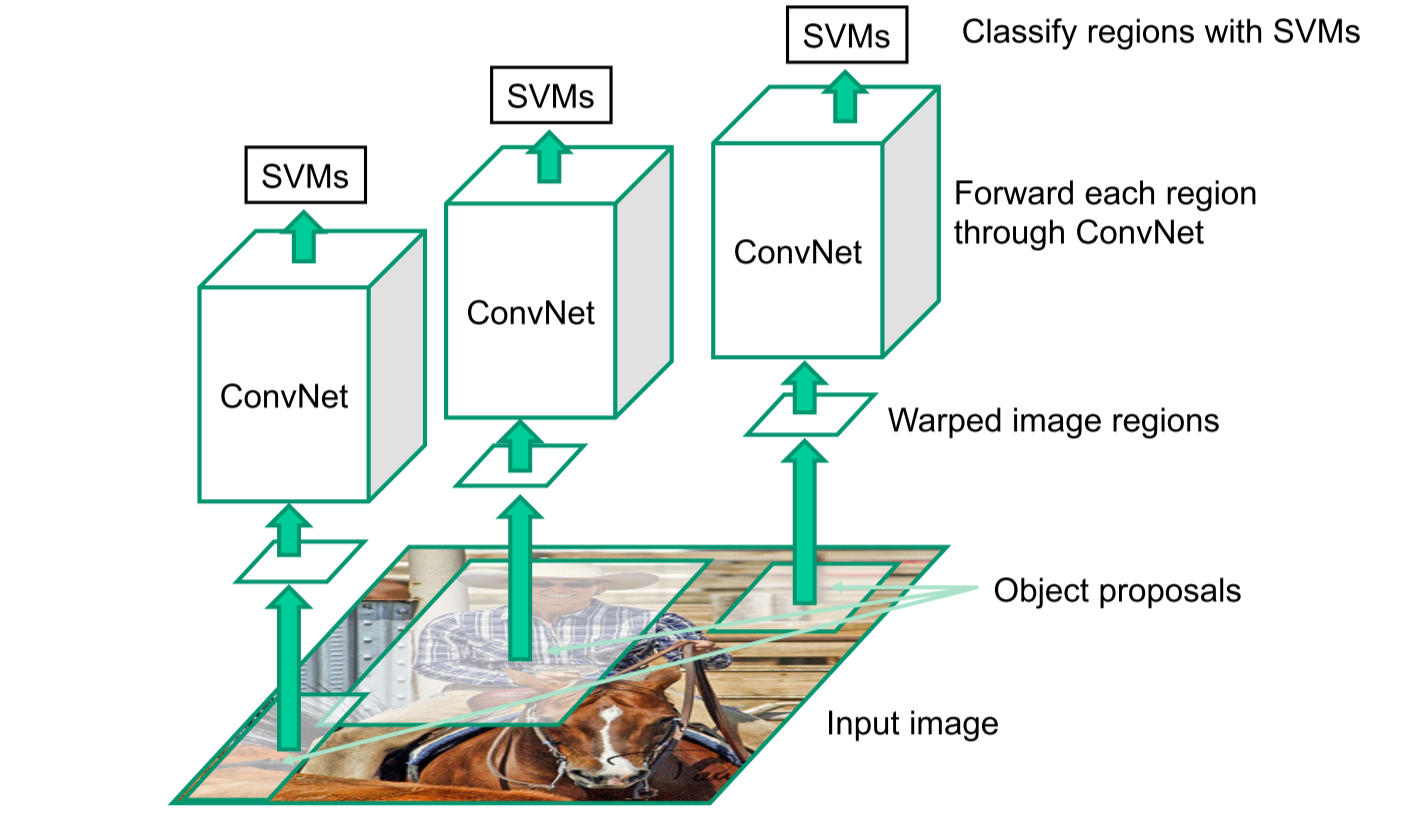
\includegraphics[width=\columnwidth]{pictures/R-CNN}
Pros
\begin{itemize}
	\item Accurate!
	\item Any deep architecture can immediately be plugged in
\end{itemize}
Cons
\begin{itemize}
	\item Ad hoc training objectives
	\begin{itemize}
		\item Fine-tuning network with softmax classifier (log loss)
		\item Train post-hoc linear SVMs (hinge loss)
		\item Train post-hoc bounding-box regressions (least squares)
	\end{itemize}
	\item Training is slow (84h), takes a lot of disk space
	\item Inference (detection) is slow
\end{itemize}
\subsubsection{Fast R-CNN}
Full Image first through ConvNet and afterwards Region selection
\subsection{Detection: a star model}
Recognition of object categories

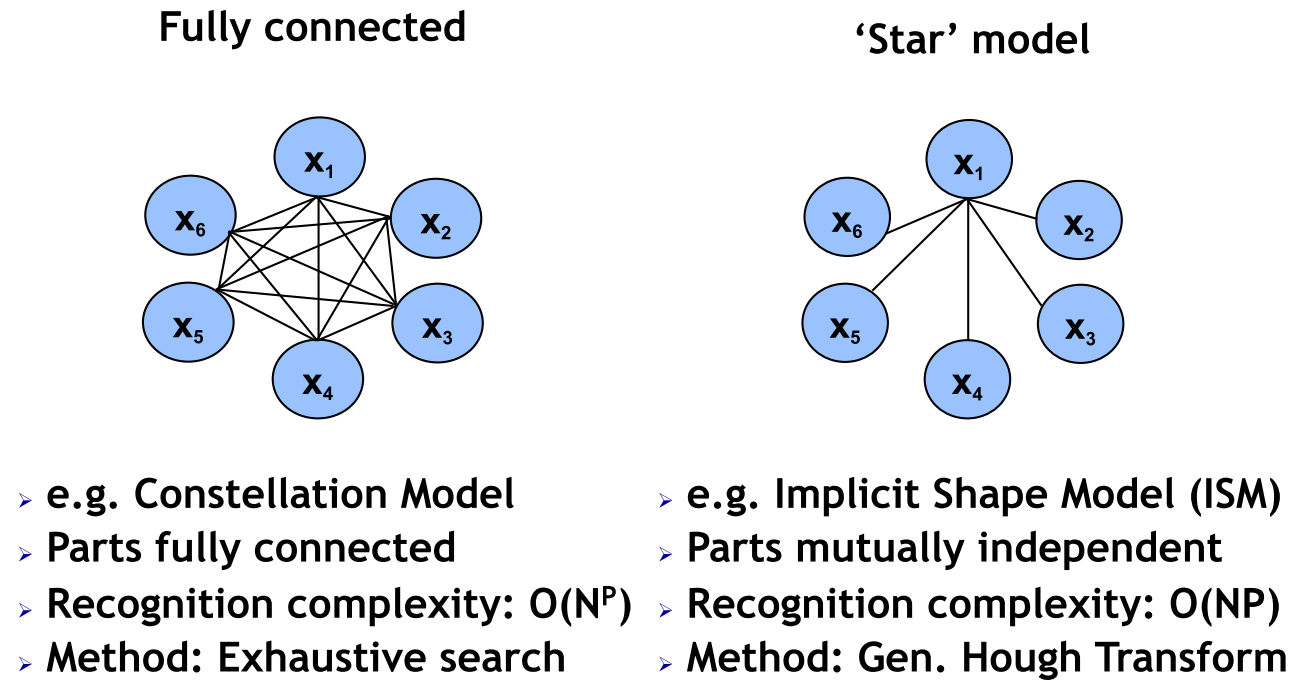
\includegraphics[width=\columnwidth]{pictures/star_models}

\subsubsection{Implicit Shape Model}
Visual vocabulary is used to index votes for object position [a visual word = a “part”].
Objects are detected as consistent configurations of the observed parts (visual words).

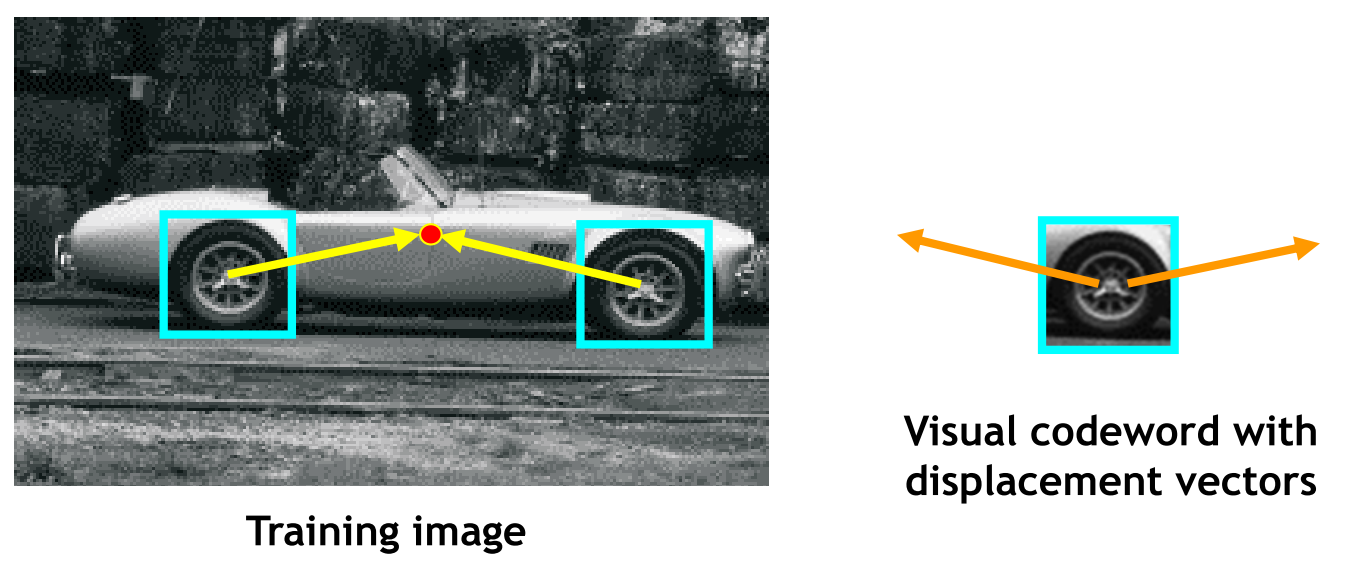
\includegraphics[width=\columnwidth]{pictures/ISM}
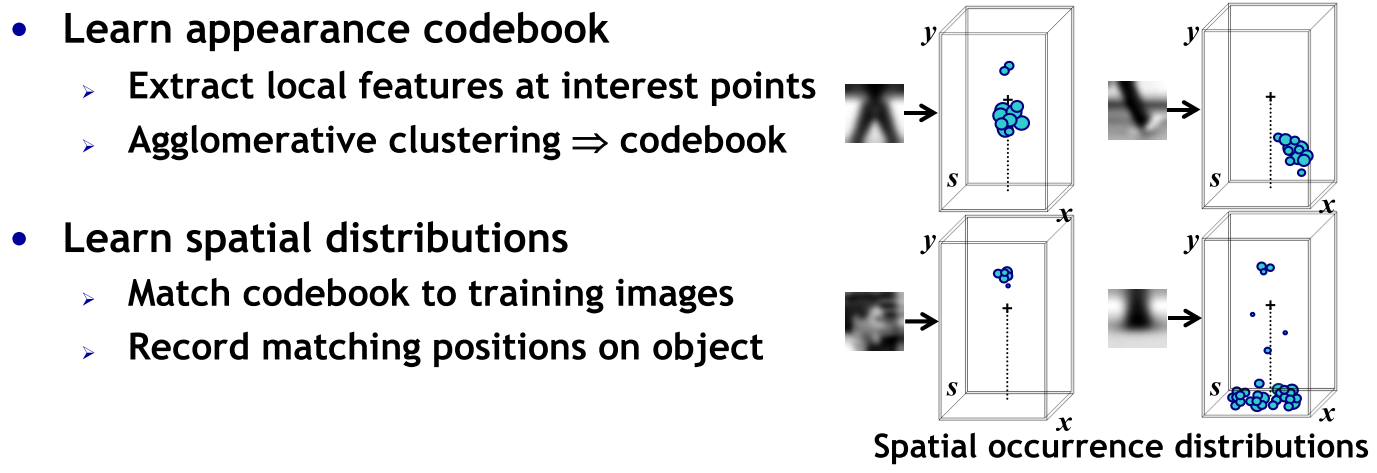
\includegraphics[width=\columnwidth]{pictures/ism_spatial}


Pros:
\begin{itemize}
	\item Works well for many different object categories – Both rigid and articulated objects
	\item Flexible geometric model – Can recombine parts seen on different training examples
	\item Learning from relatively few (50-100) training examples
	\item Optimized for detection, good localization properties
\end{itemize}
Cons:
\begin{itemize}
	\item Needs supervised training data – Object bounding boxes for detection \& Segmentations for top-down segmentation
	\item Only weak geometric constraints – Result segmentations may contain superfluous body parts.
	\item Purely representative model – No discriminative learning
\end{itemize}
